\documentclass{article}

\usepackage[T1]{fontenc}
\usepackage[utf8]{inputenc}
\usepackage[italian]{babel}
\usepackage[colorlinks]{hyperref}
\usepackage{framed}
\usepackage{graphicx}
\usepackage[inkscapeformat=png]{svg}
\usepackage{hyperref}% http://ctan.org/pkg/hyperref
\hypersetup{%
  colorlinks = true,
  linkcolor  = black
}

\title{Documentazione del progetto di \\ Ingegneria del Software}
\author{Gabriele Faustinoni (VR457626) \\ Alessandro Lorini (VR455950) \\ Giovanni Tosini (VR457575)}
\date{}

\begin{document}

    \begin{titlepage}
        \maketitle
    \end{titlepage}

    \newpage
    \tableofcontents
    \newpage

    \section{Note introduttive}

    Il sistema in questione è stato creato per un'azienda interinale 
    per la gestione dei lavoratori stagionali.

    \section{Requisiti}

    Gli operatori dell'agenzia per poter lavorare avranno necessità di essere in possesso delle loro credenziali, che verranno create appositamente dagli sviluppatori del suddetto sistema.

    I lavoratori stagionali interessati potranno presentarsi agli sportelli dell'agenzia per farsi registrare, oppure, se già presenti in archivio, per aggiornare il loro storico lavorativo degli ultimi 5 anni.
    La registrazione consiste nel salvataggio dei dati del lavoratore

    \begin{itemize}
        \item nome
        \item cognome
        \item luogo e data di nascita
        \item nazionalità
        \item indirizzo di residenza
        \item telefono cellulare (non obbligatorio)
        \item lingue parlate
        \item patente e se automunito
        \item eventuali esperienze precedenti (non sono necessariamente i lavori fatti negli ultimi 5 anni)
        \item periodi e zone di disponibilità per lavorare
        \item una persona da contattare per eventuali emergenze, della quale saranno necessari: 
        \begin{itemize}
            \item nome;
            \item cognome;
            \item indirizzo e-mail;
            \item numero di telefono.
        \end{itemize}
    \end{itemize}

    L'aggiornamento del loro storico lavorativo consiste nella semplice ricerca del lavoratore (se presente in archivio) tramite nome, cognome e data di nascita e l'inserimento di:

    \begin{itemize}
        \item periodo in cui ha lavorato;
        \item nome azienda;
        \item luogo di lavoro;
        \item retribuzione lorda giornaliera;
        \item mansioni svolte.
    \end{itemize}

    I dipendenti dell'agenzia inoltre possono usare una funzione che permetterà di ricercare una figura lavorativa specifica (usando l'inclusione obbligatoria di tutti i parametri), oppure di una figura con solo alcuni dei criteri necessari. Una volta fatta la ricerca l'elenco verrà stampato in un'apposita finestra. 
    
    I parametri della funzione ricerca sono:

    \begin{itemize}
        \item nome;
        \item cognome;
        \item periodo di disponibilità;
        \item città di residenza;
        \item patente e se automunito;
        \item mansioni;
        \item lingue parlate.
    \end{itemize}

    \section{Scenari d'uso}

    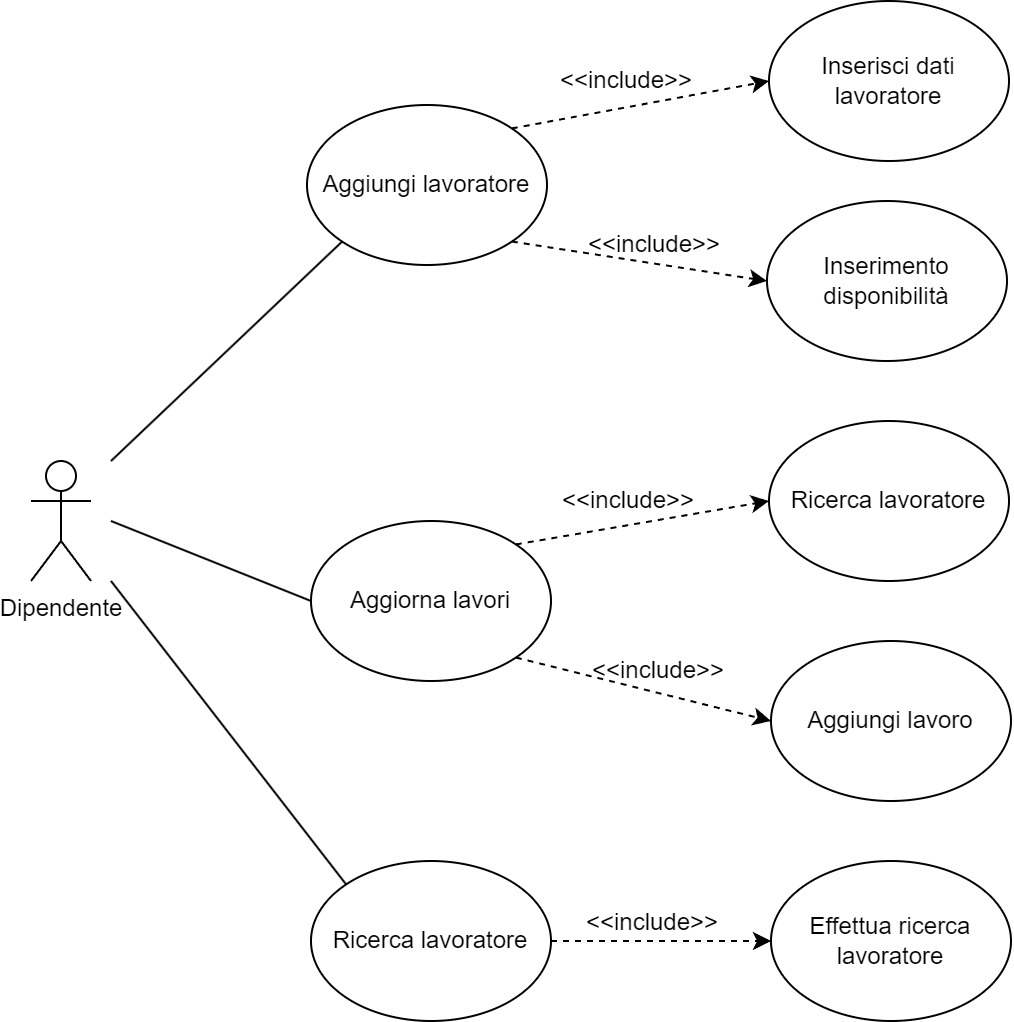
\includegraphics[width=0.9\textwidth]{casi_uso.jpg}

    \subsection{Aggiunta lavoratore da parte del dipendente dell'agenzia}

    \begin{framed}{}
        \begin{itemize}
            \item[] \textbf{Attori}: dipendente agenzia
            \item[] \textbf{Precondizioni}: il dipendente deve essersi autenticato
            \item[] \textbf{Passi}: \begin{enumerate}
                \item Clicca su "\textbf{Aggiungi lavoratore}"
                \item Inserisce dati del lavoratore:
                \begin{itemize}
                    \item dati anagrafici
                    \item contatti (numero telefonico facoltativo)
                    \item patente di guida e se auto-munito
                    \item lingue parlate
                    \item esperienze di lavoro (facoltative)
                    \item contatto persona d'emergenza
                \end{itemize}
                \item Inserimento comuni e periodi di disponibilità a lavorare (possono esserne inseriti più di uno)
                \item Salvataggio delle varie disponibilità premendo su "\textbf{Salva e continua}"
                \item Salvataggio del lavoratore premendo su "\textbf{Exit}"
                \item Ritorno all'interfaccia di partenza
            \end{enumerate}
            \item[] \textbf{Post-condizioni}: il lavoratore è stato salvato.
        \end{itemize}
    \end{framed}

    \includesvg[height=5in]{aggiungi_lavoratore.svg}

    \subsection{Aggiorna lavori}

    \begin{framed}
        \item[] \textbf{Attori}: dipendente agenzia
            \item[] \textbf{Precondizioni}: il dipendente deve essersi autenticato
            \item[] \textbf{Passi}: \begin{enumerate}
                \item Clicca su "\textbf{Aggiorna lavori}"
                \item Ricerca il lavoratore tramite nome, cognome e data di nascita
                \item Inserimento di:
                \begin{itemize}
                    \item periodo;
                    \item nome azienda;
                    \item luogo di lavoro;
                    \item retribuzione lorda giornaliera;
                    \item mansioni svolte.
                \end{itemize}
                \item Salvataggio premendo su "\textbf{Salva tutto}"
                \item Ritorno all'interfaccia di partenza
            \end{enumerate}
            \item[] \textbf{Post-condizioni}: il lavoro è stato aggiornato.
    \end{framed}

    \includesvg[height=5in]{aggiorna_lavori.svg}

    \subsection{Ricerca lavoratore}

    La ricerca del lavoratore può essere eseguita considerando tutti i parametri inseriti o almeno uno di essi, cliccando sugli appositi pulsanti. Premendo su "\textbf{Reset parametri}" è possibile cancellare tutti i parametri inseriti.

    \begin{framed}
        \item[] \textbf{Attori}: dipendente agenzia
            \item[] \textbf{Precondizioni}: il dipendente deve essersi autenticato
            \item[] \textbf{Passi}: \begin{enumerate}
                \item Clicca su "\textbf{Ricerca lavoratore}"
                \item Ricerca il lavoratore tramite:
                \begin{itemize}
                    \item dati anagrafici;
                    \item periodo di disponibilità;
                    \item patente e se automunito;
                    \item mansioni svolte;
                    \item lingue parlate.
                \end{itemize}
                \item Premendo su "\textbf{Ricerca}" si visualizzeranno nome, cognome e data di nascita dei lavoratori con le caratteristiche indicate
                \item Premendo "\textbf{Exit}" si fa ritorno all'interfaccia di partenza
            \end{enumerate}
            \item[] \textbf{Post-condizioni}: elenco dei lavoratori.
    \end{framed}

    \includesvg[height=5in]{ricerca_lavoratori.svg}   

    \section{Diagramma delle attività}

    Si fa presente che il seguente diagramma delle attività è stato concepito senza considerare la possibilità di ripetere
più volte, o annullare prima del compimento, le attività qui rappresentate. Lavorare senza questa
assunzione avrebbe portato ad un diagramma finale decisamente più complesso e poco comprensibile; cosa che
sarebbe risultata controproducente al fine del diagramma delle attività.

    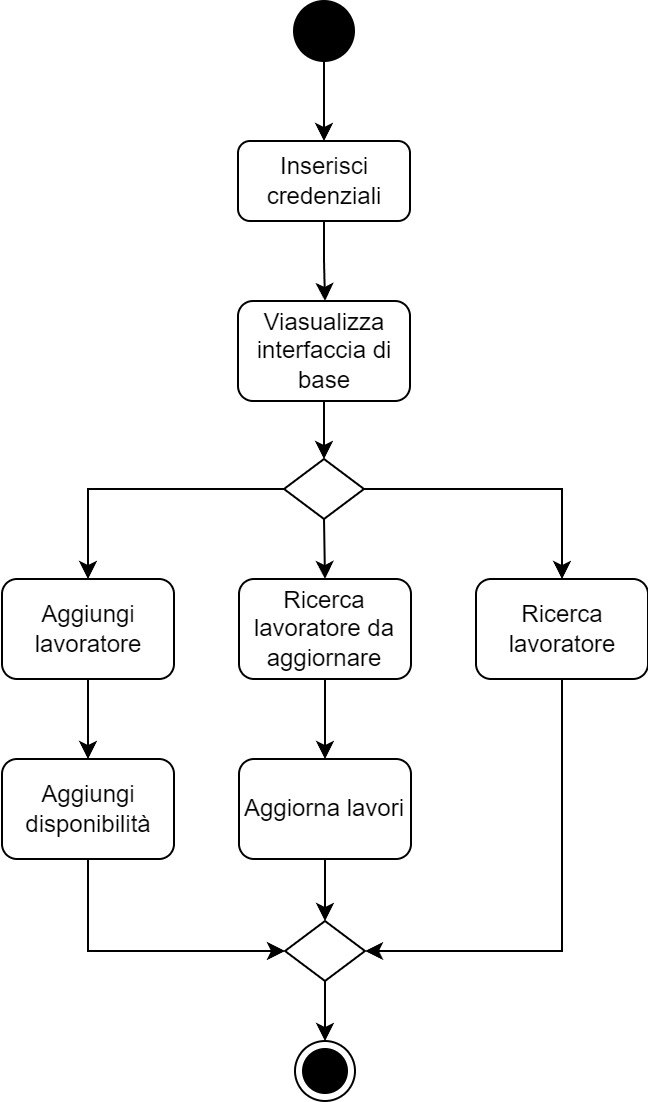
\includegraphics[width=0.9\textwidth]{diagramma_attività.jpg}

    \section{Sviluppo}

    \subsection{Scelte progettuali}

    Per il progetto sono state fatte le seguenti scelte progettuali:
    \begin{itemize}
        \item le patenti sono generalizzate, senza inserire le sotto categorie ed escludendo patenti speciali;
        \item non c'è un controllo effettivo se la città di nascita e/o di residenza esistano veramente e siano geograficamente corrette, si lascia tale responsabilità all'operatore;
        \item i comuni per le disponibilità sono ridotti ai soli centri più popolosi;
        \item per i lavori stagionali si è presa una lista ufficiale da Decreto del Presidente della Repubblica 7 ottobre 1963, n. 1525;
        \item i lavori messi di default non possono essere modificati dai dipendenti dell'agenzia, ma solo dagli sviluppatori del software;
        \item nella schermata di ricerca c'è la possibilità di eliminare tutti i parametri inseriti precedentemente tramite un comodo pulsante;
        \item si è scelto di usare il Date Picker per la gestione delle date;
        \item se i parametri per la ricerca non vengono specificati non saranno considerati;
        \item il salvataggio permanente dei dati è stato gestito tramite file JSON;
        \item eventuali credenziali per nuovi dipendenti dell'agenzia potranno essere aggiunte solo dagli sviluppatori;
        \item il sistema accetta lavoratori con un'età maggiore o uguale a 14 anni;
    \end{itemize}

    \subsection{Modelli architetturali e progettazione ad alto livello}

    Per il progetto la scelta migliore che si poteva fare in ambito di modello architetturale era per forza il modello MVC, perché permette una mantenibilità non indifferente, grazie alla divisione delle classi tra Model, View e Controller. Se in futuro si volesse cambiare il metodo di salvataggio permanente dei dati da JSON a qualcos'altro si dovrà solamente mettere mano alla classe Model. Per l'interfaccia utente si è scelto di usare JavaFX, che si presta molto all'applicazione con l'architettura MVC.
    \begin{itemize}
        \item[] \textbf{Model}: gestisce i dati del sistema e si occupa di salvarli. Ogni volta che sarà necessario leggere o scrivere qualcosa sul file JSON verrà sempre usato un metodo della classe Model.
        \item[] \textbf{View}: l'interfaccia grafica dell'utente, specifica ciò che si potrà vedere a schermo.
        \item[] \textbf{Controller}: fa da punto di raccordo tra il View e il Model: accetta l’input dell’utente e lo converte in comandi per Model e View.
    \end{itemize}

    \subsection{Diagramma delle classi}

    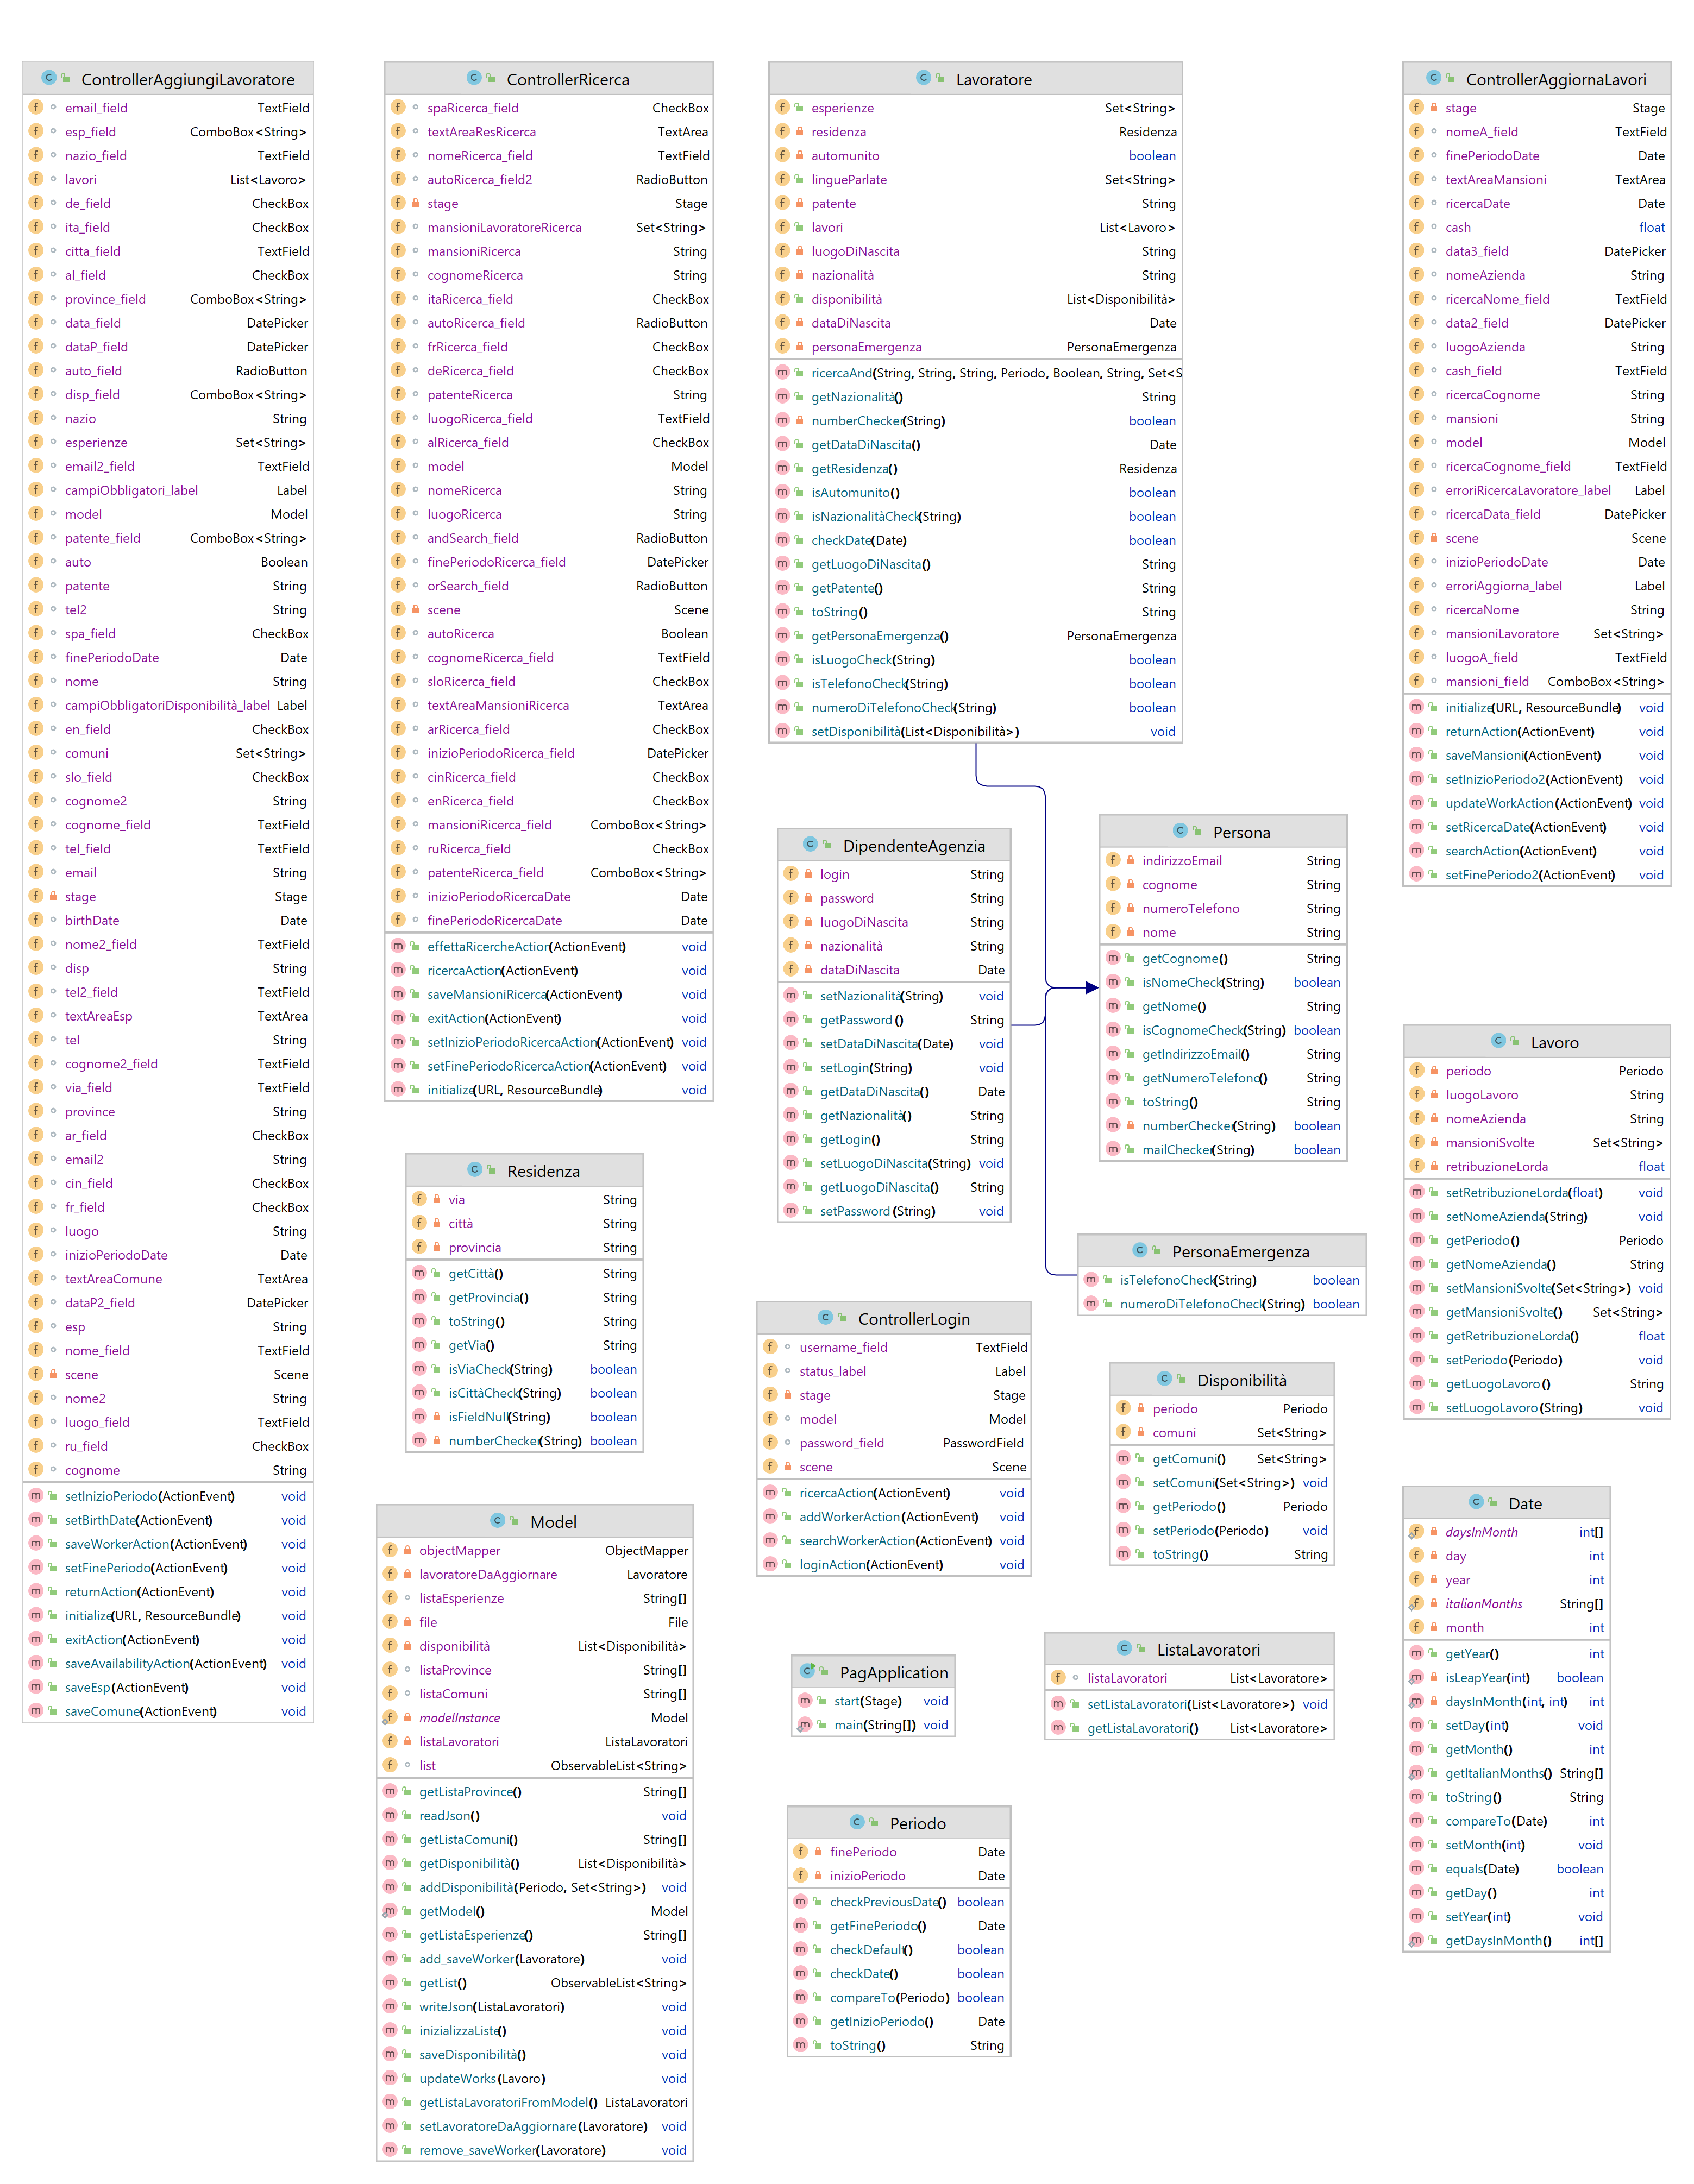
\includegraphics[width=\linewidth]{class diagram.png}

    Il class diagram corrisponde alla vista del Model e del Controller.
Possiamo osservare che le classi sono state istanziate nella sintassi UML e contengono i vari metodi ed attributi.

Per quanto riguarda i campi dei controller, alcuni vengono utilizzati per consentirci di estrapolare dall'interfaccia grafica i dati inseriti dall'utente.
Notiamo che la classe Model è responsabile nella gestione dei dati dei lavoratori, ci permette di salvarli e di leggerli da un file JSON. In sostanza si occupa di tutta la gestione dei dati da e verso l'applicativo. Per poter utilizzare i suoi metodi, i controller usufruiranno del getModel() che si occuperà di ritornare l'istanza del model, in modo che i controller possano utilizzare i suoi metodi per leggere o scrivere i dati.

Notiamo che i controller che sono responsabili delle varie operazioni richieste dall'utente non sono in comunicazione tra loro. Questo dipende dall’implementazione adottata da JavaFX.

Per definire le varie schermate abbiamo usato i file FXML, una tecnica di sviluppo che consente di velocizzare la creazione dell’interfaccia grafica. 
La classe PagApplication è la classe dove viene inizializzato lo stage di JavaFX, in cui viene caricata una scena (la schermata di Login),
in cui i metodi dovranno essere istanziati per caricare una nuova schermata nella finestra esistente.

Infine possiamo notare una gerarchia tra le classi DipendenteAgenzia, Lavoratore, PersonaEmergenza e Persona, dove quest'ultima è la classe padre mentre le altre sono classi figlio che ereditano tutti i metodi e gli attributi presenti nella classe padre.



    \subsection{Sequence Diagram}

    Da fare?

    \subsection{Design Pattern}

    Durante la progettazione sono stati implementati due design pattern: l'iterator pattern e il singleton.

    \begin{itemize}
        \item[] \textbf{Iterator Pattern}: è utilizzato internamente da linguaggio Java e dalla sua
libreria standard, pertanto è stato implicitamente utilizzato. Un chiaro esempio di utilizzo di
questo pattern è trovabile nei metodi AGGIUNGERE NOMI METODI, che vengono utilizzati per leggere la lista dei lavoratori e per fare ricerche al suo interno.
        \item[] \textbf{Singleton Pattern}: è stato applicato per assicurarci che la classe Model, ovvero la classe con il compito di gestire i dati, venisse creata un'unica volta. In modo che quando ci si interfacciava con un metodo di scrittura/lettura lo si facesse sempre con lo stesso oggetto.
    \end{itemize}

    \subsection{Pianificazione e organizzazione del processo di sviluppo}

    Come prima cosa si è abbozzato un diagramma dei casi d'uso, in modo da capire cosa venisse richiesto ad un livello molto alto. Da quel diagramma poi siamo passati a definire nello specifico i singoli casi, con l'eventuale sequence diagram. La metodologia di progettazione che abbiamo applicato si può definire in assoluto Agile, partendo dai requisiti strettamente necessari e man mano modificando/aggiungendo parti o rimuovendo altre non necessarie. Quando sorgeva un problema il gruppo intero si concentrava per risolvere, come i problemi di dipendenze per le librerie esterne che volevamo applicare.
    
    L'obiettivo principale per il progetto era di scrivere il codice necessario per farlo funzionare, anche solo una bozza, per poi concentrarsi sui possibili controlli, che sono stati implementati verso la fine del lavoro.


    Per il version control si è deciso di usare GitHub, per permettere di avere un controllo delle modifiche fatte ed eventualmente correggere errori andando a recuperare versioni precedenti.

    Per la scrittura effettiva del codice si è deciso di optare per il pair programming, in parte obbligati perché i membri del gruppo abitano a parecchia distanza l'uno dall'altro e quindi le possibilità di vedersi di persona erano poche, ma anche perché si voleva lavorare ad ogni singola parte del processo e poi scegliere congiuntamente. Una persona condivideva lo schermo tramite Zoom e scriveva, mentre gli altri controllavano cosa si doveva fare e correggevano eventuali errori, oltre a decidere le ottimizzazioni necessarie.

    \subsection{Librerie di terze parti}

    Il linguaggio con cui abbiamo deciso di fare l'intero progetto è Java. Il sistema usato per gestire le librerie di terze parti è Maven, già integrato nell'IDE utilizzato per lavorare, ovvero IntelliJ. 
    
    Come librerie abbiamo scelto di usare:
    \begin{itemize}
        \item[] \textbf{JavaFX} per la parte grafica del progetto tramite l'aiuto di SceneBuilder, il quale permetteva di creare file FXML usati da JavaFX, evitando di dover creare manualmente tutte le scene;
        \item[] \textbf{Jackson databind} per la serializzazione e deserializzazione dei file JSON, scelto come tipologia di file per il salvataggio permanente dei dati.
    \end{itemize}

    \section{Test e validazione}

    Questa parte importante della progettazione è avvenuta dopo aver creato lo scheletro del progetto e sono stati eseguiti controlli sia dagli sviluppatori che da altri volontari.

    \subsection{Test manuali degli sviluppatori}

    \begin{itemize}
        \item[] \textbf{Validazione del login}: al sistema possono accedere solo gli utenti in possesso di credenziali. In caso di errate credenziali il sistema manderà un messaggio di errore.
        \item[] \textbf{Verifica parametri}: tale controllo avviene dopo l'invio dei dati e verifica che i parametri obbligatori siano stati inseriti tutti e che rispettino il campo in cui sono stati messi (esempio: nel campo nome e cognome non si possono indicare numeri, oppure nel campo e-mail c'è una regex che verifichi il formato di default degli indirizzi e-mail). In caso di errore il sistema avviserà con un messaggio evidenziando in rosso i campi con i dati errati.
        \item[] \textbf{Coerenza dei dati}: il sistema verifica che i periodi per la disponibilità siano successivi alla data di registrazione, che l'inizio sia precedente alla fine, l'eta del lavoratore rientri nei parametri specificati nelle scelte progettuali e che le esperienze passate non siano più vecchie di 5 anni.
    \end{itemize}

    \subsection{Test eseguiti dagli utenti}

     Una volta terminato lo sviluppo, questi test sono stati eseguiti da persone esterne senza dire loro come funzionava il programma, lasciando che fosse il sistema a correggerli nel caso di errori e annotando eventuali problemi che sorgevano per sistemarli successivamente.
    


\end{document}


